\documentclass{article}
\usepackage{url,amsfonts, amsmath, amssymb, amsthm,color, enumerate, graphicx, parskip, color}
\graphicspath{{../images/}{../graphs/}}
% Page layout
\setlength{\textheight}{9in}
\setlength{\columnsep}{2.0pc} %pc = pica = 12pt
\setlength{\textwidth}{6.5in}
\setlength{\topmargin}{0pt}
\setlength{\headheight}{0.0in}
\setlength{\headsep}{0.0in}
\setlength{\oddsidemargin}{0in}
\setlength{\evensidemargin}{0in}
\setlength{\parindent}{0pt}
\setlength{\parskip}{1em}
\frenchspacing
% Macros for course info
\newcommand{\shortname}{Kar Epker}
\newcommand{\fullname}{Karthic N. Epker}
%====header======
\newcommand{\header}[4]{
%\renewcommand{\thetheorem}{{#2}.\arabic{theorem}}
\vspace{-2ex}
\begin{flushleft}
{\large \shortname} \hfill {#1} \\
\textsc{#2} \hfill{#3} \\
\vspace{-1ex}
\hrulefill
\end{flushleft}
\begin{center}

{\LARGE #4}\\
\end{center}
\vspace{3ex}
}
\begin{document}
\header{Professor Evrard/Dr. Popov/Professor Orr}{Physics 160}{2012-04-18}{Modeling the deformation of a golf ball}
%%%%%%%%%%%%%%%%%%%%%%%%%%%%%%%%%%%%%%%%%%%%%%%%%

\begin{abstract}

The deformation of objects as a result of force is one of its important ef\mbox{f}ects, but because of its chaotic nature, cannot be described easily with a set of equations. While many deformations occur in the world, a particular case, that of a golf ball being hit by a club, was explored. In order to explore this motion computationally, a ball-spring model of the golf ball was made. The ball-spring model uses a clever substitution in the definition of Young's modulus to calculate a ``spring constant'' for two points. Geodesic spheres were used to place individual ``balls'' (henceforth referred to as ``particles'') evenly on the surface of nested geodesic spheres. The particles were then connected to each other using a set of springs, whose constant was found using the Young's modulus for butadiene rubber, a common material for the inside of golf balls. Qualitatively, the end simulation appeared to agree with existing videos of a golf ball being hit in slow motion. Quantatively, the velocity of the center of mass of the ball corresponded with measured values, as did the time scale for the wave which moves through the ball, but the spin was found to greatly exceed the measured values for spin of golf balls. It was concluded that the ball-spring model of solids is appropriate for simulating a golf ball. Further work may seek to improve the accuracy of the model.
\end{abstract}

\section{Introduction}

The deformation of the objects under a force is dif\mbox{f}icult to study in an elementary calculus based physics course is hard to study as deformation can be difficult to quantify and varies based on the shape of an object. Deformation does, however, take place in physical systems, as the bounce of a ball will confirm. Deformation, and the composition of objects also relate to how energy will be spread during a collision, determining the objects behavior after the collision \cite{whybounce}. While there are a myriad of collisions that occur in nature, here, the man-made collision of a golf club with a golf ball will be modeled. Golf has been played since the 1400s, \cite{history} and as a popular sport today, will provide a relevant and interesting example of examining deformation. Golf balls have also been the subject of many patents, (simply visit \url{http://patft.uspto.gov/} and perform a query for ``golf ball'' to see this) meaning that there is plenty to investigate. While the most outwardly striking di\mbox{f}ference between a golf ball and a normal sphere are the dimples on golf balls, because simulating this would involve modeling the flow of the air over a golf ball, this aspect of the golf ball will be ignored in favor of something slightly easier to approximate.

The collision between a golf ball and a golf club proves to be better material for simulation. While golf balls can come between one and four pieces \cite{general}, a two piece golf ball will be simulated for simplicity. As golf is played with a variety of clubs with dif\mbox{f}erent lofts depending on the type of shot intended to be hit, multiple lofts will be investigated in this simulation. While no club (besides the putter) has a $0^{\circ}$ loft, this will be used as a baseline case as there should be no spin generated by a club with this loft. Clubs with lofts of up to $60^{\circ}$ will be investigated, as this a fairly standard degree value for a wedge. A variety of dif\mbox{f}erent swing speeds will also be investigated. The RE/MAX World Long Drive Championship from 2009 will provide the upper end of the data, while the lower end will be done by estimation.

The ball-spring model of solids will be used to model the golf ball. This model uses the fact that the formula for the spring-constant may be substituted into the formula for Young's modulus. The ball-spring model is an approximation that can be used to accurately simulate solids with a limited amount of computational resources. This approximation may be used to investigate deformations and propagations of disturbances like sound, through objects. For this reason, it is perfect for the use of modeling with a golf ball, as it allows disurbances and deformation to be seen in the ball. For more information on the ball-spring model of solids, see Chapter 4 in \textit{Matter \& Interactions} \cite{sherwood}

While there are many outcomes to consider when hitting the golf ball, the simulation will be structured to revolve around the idea of changing the loft of the club. If the loft is increased, wil the ball spin more? How will the velocity change? Also, how well do the results from the simulation correspond to real measurements?

\section{Methods}

There are two major design challenges in designing the simulation described above. They are listed below: \begin{enumerate}[1.]
\item Designing an appropriate ball-spring model of a golf ball
\item Applying the physics correctly
\end{enumerate}
The solution to each of these problems is discussed in the subsections below:

\subsection{Designing the model}

\subsubsection{Making each layer}
With current computing technologies, it is impossible to simulate all of the atoms in a golf ball, so an approximation must be used, and a subset of represetative points must be taken instead. These points should be distributed equally at a given radius, as each shell of a golf ball has a uniform density. Also, the ball must be solid; this entails having at least two or three nested spheres (these will be called ``layers''). The outermost layer must have an radius equal to the radius of the actual golf ball. Furthermore, the number of particles in each layer must be smaller than the number of particles in the layer outside it so the ball's density does not decrease as it's radius becomes smaller.

To create the uniform model of the ball and sphere, nesting geodesic spheres were used. Geodesic spheres (``Spaceship Earth'' in Epcot, Disney World is a famous example), solve this problem by allowing the placement of a finite number of points uniformly on the sphere. An algorithm for creating geodesic spheres is provided by Adrian Rossiter \cite{packinon}. His code in Python outputs a set of points for a geodesic sphere given three parameters: A type of base polyhedron to use (a regular tetrahedron, a regular octahedron, a regular icosahedron, or a single equilateral triangle), a frequency $\in \mathbb{Z^{+}}$ or class type specified by $a, b \mid a, b \in \mathbb{Z^{+}} \cup \{0\}$. This algorithm will be referred to as \texttt{packinon}.

For the purposes of this model, $a$ and $b$ are irrelevant, they solely determine the orientation of the golf ball. Similarly, while the base polyhedron may does have some ef\mbox{f}ect on the way the sphere looks, since the model needed only requires a single way to distribute points on a sphere, an icosahedron was chosen as the base polygon. The value of frequency is somewhat more important. The frequency of sphere, which is equivalent to the number of points between each vertex not including the vertices, allows layers to be nested while reducing the number of points.

To form a set of layers that could be connected to each other well, powers of two were chosen as frequencies. This allows each set of layers with frequences of decreasing powers of two. Let layers be denoted by $L_i, 1 < i < n, n = \text{number of layers desired}$ and let $f_{i}$ be the corresponding frequency for each layer. $f_{1} = -1$, which we define to be a geodesic sphere that consists of a single point at the center of the sphere. $f_{2} = 0, f_{3} = 1, f_{4} = 2, \ldots, f_{n} = n - 2$. This choice of frequencies for nesting the layers provides a convenient way to connect $L_{i}$ to $L_{i + 1}$ as will be described later, in addition to providing a clean nesting pattern.

While much of the math completed by \texttt{packinon} was irrelevant to this physics simulation, some knowledge of the order in which the particles were placed by the algorithm was needed in order to create an algorithm connect adjacent particles. \texttt{packinon} initially adds the twelve vertices of an icosahedron for any frequency of geodesic sphere to the list of points. Then, points on each of the 20 ``faces'' of the geodesic sphere are added to the list. While the exact order in which points are added to the list is somewhat more involved, this information was needed to connect particles correctly.

\subsubsection{Connecting the particles in the model}
After generating the points on the surface of each sphere using the provided algorithm, two operations must be performed to complete the ball-spring model. 
\begin{enumerate}
\item Each point $v$ on $L_{i}$ must be connected to its adjacent points on $L_{i}$. \label{item:neighbors}
\item Each point $v$ on $L_{i}$ must be connected to its adjacent points on $L_{i + 1}$ and $L_{i - 1}$ (if they exist). \label{item:nested}
\end{enumerate}

While most of the code discussed has been and will be abstracted from implementation in a specific language, here a discussion is made of how adjacent points were represented in VPython because the implementation is made more elegant by a few tricks not presented or necessary in past simulations. A class \texttt{Spring} was defined to represent each spring. Every \texttt{Spring} has variables \texttt{constant} and \texttt{neighbor}, and \texttt{rest}, containing, respectively, the spring constant, the index of the neighbor this Spring is connecting, and the rest length of the spring. An array of \texttt{Spring}s (called \texttt{springs}) was made for each particle, corresponding to how many particles were connected to it.

To connect each particle to its adjacent particles (sometimes called ``neighbors''), first, operation \ref{item:neighbors} was considered. While this task can be completed in linear time (constant time for each particle), as the position of each particle is put in an array in an orderly way, this proves to be algorithmically complex and does not of\mbox{f}er enough of a real world time benefit for relatively small value of $f_{n}$. The fact that the model must only be constructed once outside of the simulation-loop, further justif\mbox{i}es the use of a slower but easier to program connection algorithm. Therefore, to connect each particle to its neighbors, a threshold for whether the balls are neighbors is set. 

First, a base threshold is determined by the distance between two balls that are known to be neighbors. As it was known that after the first 12 particles are placed, points on each face are created, the 13\textsuperscript{th} and 14\textsuperscript{th} particles on each layer are adjacent. If the layer has less than 13 particles, then it can only be an icosahedron, in which case vertices will be adjacent to each other. For the case with just an icosahedron, the base threshold was set to the distance between the 4\textsuperscript{th} and 5\textsuperscript{th} particles, which were known by observation to be adjacent.

Second, the base threshold was multiplied by a constant $\texttt{NEIGHBOR\_TOLERANCE} > 1$ to determine final threshold, which accounts for the fact that adjacent points are not perfectly equally and the distance between any two may be slightly greater than the base threshold found. Currently, $\texttt{NEIGHBOR\_TOLERANCE} = 1.15$. Then, for each particle in the layer, every other particle in the layer is looped over to determine if it is adjacent. If the distance is less than the threshold, it is considered adjacent.

One final note of interest in the implementation of connecting neighbors in the same layer comes if we consider the ``connected'' relation $C$ for any two particles $p$ and $q$. $(p, q) \in C$ if $p$ and $q$ are connected by a spring. While this relationship is symmetric, the implementation only adds one side of the relation at a time. This consideration is made for speed. This allows the pair $(p, q)$ to be added to $C$ every time, without having to check if $(p, q)$ already exists in the relation. In more concrete terms, when $q$ is found as a neighbor to $p$, a \texttt{Spring} with \texttt{index} $q$ may be added to \texttt{springs} immediately. Then, when $p$ is later found as a neighbor of $q$, a \texttt{Spring} with \texttt{neighbor} $p$ may be added to \texttt{springs} immediately without checking that the \texttt{Spring} was not added by an earlier operation. Note that this also makes a good invariant for checking that this algorithm worked.

After operation \ref{item:neighbors} was considered, operation \ref{item:nested} was considered. Determining which points in $L_{i + 1}$ and $L_{i - 1}$ to connect each point in $L_{i}$ to is slightly more dif\mbox{f}icult than operation \ref{item:neighbors}. This operation is made easier by two observations. One: The connected relation $C$ is symmetric (as discussed above). Here it is convenient to add both sides of the relation at once, then, each layer $L_{i}$ must only be connected to layer $L_{i + 1}$, it will be connected to layer $L_{i - 1}$ when layer $L_{i - 1}$ connects itself to layer $L_{i}$. Two: by choosing frequencies that are powers of two, determining which points to connect becomes simpler. Here, a figure becomes convenient to demonstrate the connections between points on layers.

\begin{figure}[h]
\centering
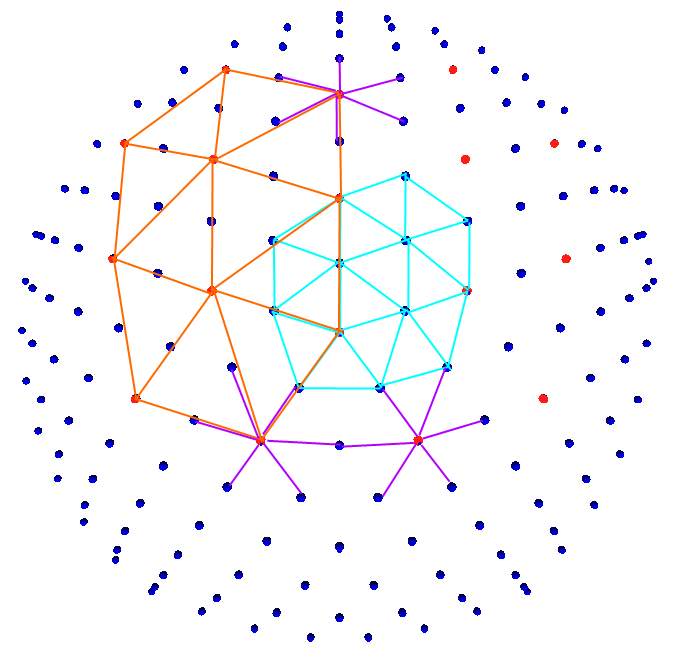
\includegraphics[width = 0.5\textwidth]{geodesic_sphere_diagram.png}
\caption{Diagram of connections in dif\mbox{f}erent layers}
\label{fig:layers}
\end{figure}

\definecolor{lightblue}{RGB}{0, 255, 255}
\definecolor{orange}{RGB}{255, 115, 16}
\definecolor{violet}{RGB}{193, 48, 255}

Figure \ref{fig:layers} demonstrates how particles placed on an inner layer $L_{i}$ correspond to those placed on a layer outside it $L_{i + 1}$. If the layer shown is layer $L_{i + 1}$, all the points colored \textcolor{red}{red} are points that will exist on layer $L_{i}$ because $2 \times f_{i} = f_{i + 1}$. If these \textcolor{red}{red} points are imaginged to be scaled down correclty, then the \textcolor{orange}{orange} lines show the connections on just layer $L_{i}$, and the \textcolor{lightblue}{light blue} lines that connect the \textcolor{blue}{blue} points represent the connections on layer $L_{i + 1}$. These two layers are connected as represented by the \textcolor{violet}{purple} lines (not all are shown). Also, the \textcolor{red}{red} point on layer $L_{i}$ will be connected to the \textcolor{blue}{blue} point directly above it on layer $L_{i + 1}$ (this \textcolor{blue}{blue} point is not shown. Therefore, every point on each layer will be connected to the appropriate points on other layers.

The actual connection algorithm for connecting dif\mbox{f}erent layers functions similarly to the algorithm that connects points within each layer. Two loops are used; the outer loops through the points in $L_{i}$, while the inner loops through the points in $L_{i + 1}$, searching for adjacent points. A base threshold is by taking the distance between the 13\textsuperscript{th} point placed in layer $L_{i + 1}$ and the 1\textsuperscript{st} point placed in layer $L_{i}$. This base threshold is then multiplied by the same \texttt{NEIGHBOR\_TOLERANCE} as given previously. If the distance between any two points is less than the calculated threshold, the points are said to be adjacent. 
\clearpage

After having solved the challenges of how to distribute points equally on each layer and how to connect appropriate points, the final model is depicted below:

\begin{figure}[h]
\centering
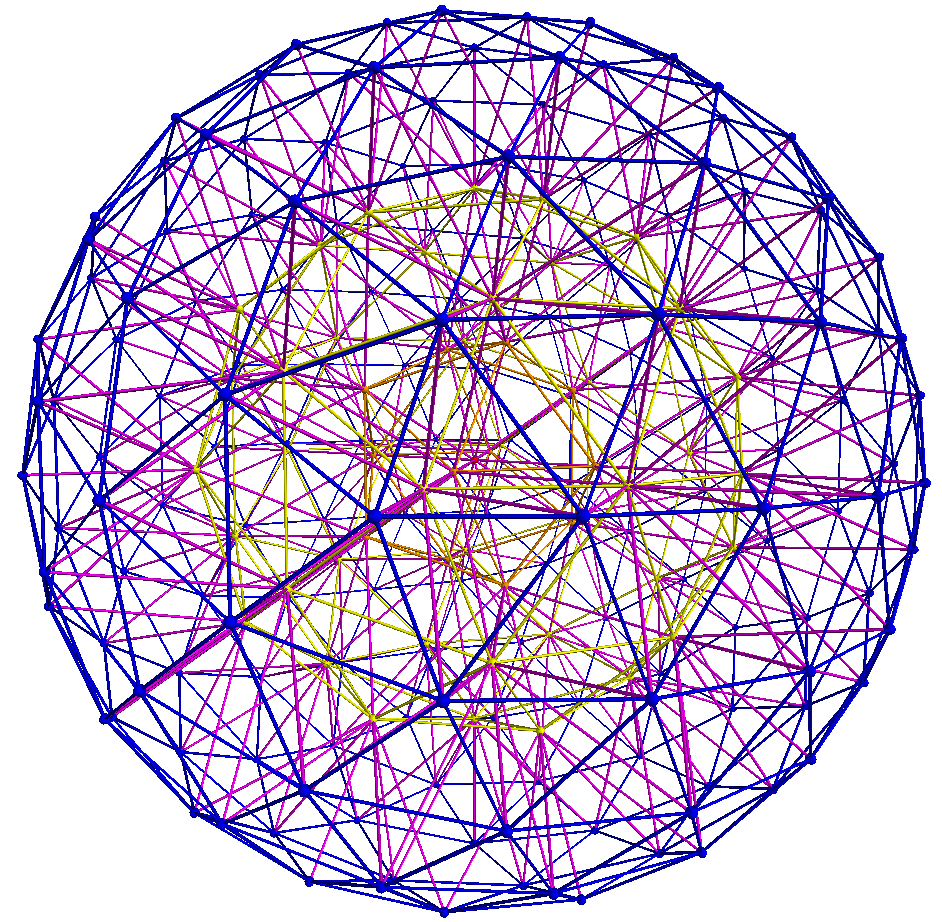
\includegraphics[width = 0.5\textwidth]{ball_spring_model.png}
\caption{Diagram of the final mode, connections between layers shown in \textcolor{violet}{purple}, connections within layer shown in other colors}
\label{fig:model}
\end{figure}

\subsection{Adding the Physics}

Key to the ball-spring model of a solid is the idea of Young's modulus, which allows a spring constant to be found. As Young's modulus is defined as $Y = \dfrac{\text{stress}}{\text{strain}} = \dfrac{F/A}{\Delta L/L}$ where $F$ the force applied on the material, $A$ is the cross sectional area the force is applied on, $Delta L$ is the change in length of the material, and $L$ is the original length of the material.. As the spring constant is defined as $k = \dfrac{F}{\Delta L}$, this may be substituted in the equation for $Y$. Solving for $k$, it is found that $k = \frac{YA}{L}$. To calculate the spring constant $k$, the \texttt{Spring} class will set \texttt{constant} = \texttt{young * (rest ** 2) / rest}, where \texttt{young} is the given Young's modulus. The cross sectional area is set to \texttt{rest ** 2} as described in Matter \& Interactions Chapter 4 \cite{sherwood}. Young's modulus for a golf ball is given by Iwatsubo, et. al \cite{young}.

Implementing the physics itself proved to be rather easy compared to creating the model. Because the club was not modeled using balls and springs, rather as a solid plane, this imposed a restriction on the system: no particle can be behind the plane. Under this assumption, instead of applying the momentum principle as used in other physics simulations, this simulation partitioned the set of all particles into two subsets $\mathcal{N}$ and $\mathcal{P}$. Particles in set $\mathcal{N}$ were assumed to be on the plane, and their positions were set to the closest point on the plane, their velocities set to the plane's velocity, and their momentum calcuated from velocity. Particles in set $\mathcal{P}$ were updated using the traditional momentum principle.

\begin{figure}[h]
\centering
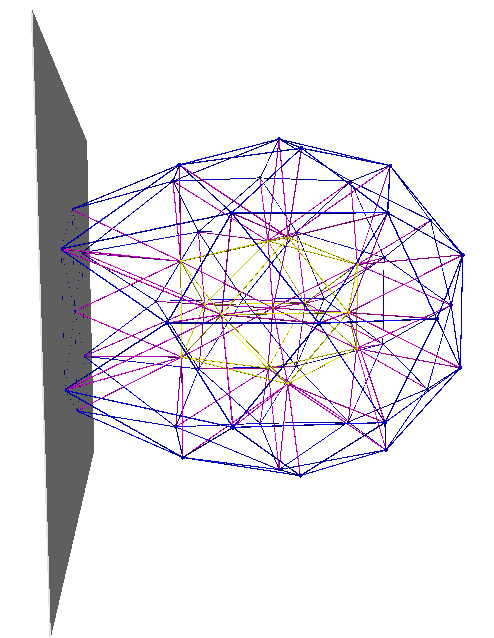
\includegraphics[width = 0.5\textwidth]{stuck_points.png}
\caption{Without a condition to allow the points to escape from the plane, they becomes stuck to it}
\label{fig:stuck}
\end{figure}

To determine which set the particles belonged in, two factors had to be taken into accout, whether the particle was within a certain range of the plane, and whether the particle was being pulled away from the plane. If any particle is behind the plane, then it is in $\mathcal{N}$. 

\section{Results}

\subsection{Qualitative}
Testing the simulation was initially done qualitatively. As the system is modeled after a phenomenon that has been somewhat well-documented in slow motion, it was possible to judge what aspects of motion should appear in the simulation. Some expected qualitative results included:

\begin{itemize}
\item Compression of the ball when it was hit
\item Spin of the ball for a lofted club
\item A ``wave'' that progressed through the ball as a result of its disturbance
\item A constant speed and spin for the ball after it left the club face
\item A disturbance that dampeneda as a result of a coef\mbox{f}icient of restitution $r < 1$
\end{itemize}

\begin{figure}[h]
\centering
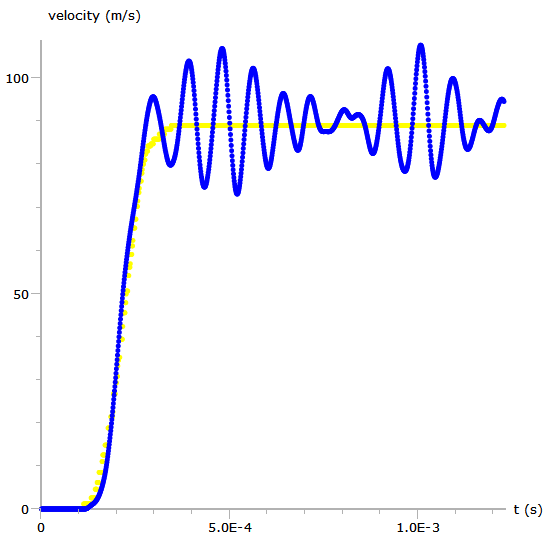
\includegraphics[width = 0.5\textwidth]{velocity_40.png}
\caption{Diagram of velocity of center of mass (yellow), and point $c$ at the center of the model}
\label{fig:velocity40}
\end{figure}

Qualitatively, the model had success. Most of the above characteristics were observed for the model. The speed of the center of mass of ball was seen to become constant (Figure \ref{fig:velocity40}) while the speed of a given point was periodic because of the disturbance passing through the ball. The last expected result, a dampening disturbance, was not observed, however. Perhaps this was a result of the short time during which the simulation was run. In actual videos of the compression of a golf ball, though, the ef\mbox{f}ect of dampening is seen almost immediately. It is also possible that the coef\mbox{f}icient of resitution should have been smaller, as coef\mbox{f}icent of restitution decreases as collision speed increases \cite{decreasing}.

\subsection{Quantitative}
Quantitative results were more dif\mbox{f}icult to obtain. While much data exist about the ball after it has left the clubhead (especially distance), data about the spin were especially dif\mbox{f}icult to find. Sample data were found through an experiment conducted with \textit{Golf Magazine} \cite{spin}.

To test the simulation, first, a club head velocity was set ($145 \text{mph} \approx 64 \text{m/s}$) the swing speed of the RE/MAX long drive winner in 2009 \cite{trackman}) loft was then by degree increments of ten and measurements were taken to find the time the ball was in contact with the club, the time it took the wave to propagate through the ball, the $x$ and $y$ components of velocity of the center of mass after the ball was no longer in contact with the club, and the spin of the ball.

Most of these components could not be measured directly from the simulation, so indirect calculation was mostly used. Calculation of the velocity of the center of mass was the most straightforward calculation, it simply calculated by summing the product of the velocity of each particle with its mass and dividing by the total mass of the particles. 

The time the ball was in contact with the club was found as a consequence of tracking the point at the center of the sphere $c$. When the ball is first hit, the velocity of this center point $c_v$ increases from zero, and when the ball leaves contact with the club, $c_v$ has a critical point. By tracking when the $c_v$ first became non-zero, and when the graph of $c_v$ had its first critical point, the time the ball was in contact with the club could be found. This solution was not perfect, however, as sometimes the graph of $c_v$ had a critical point before the ball had left contact with the club. This occurred at the higher lofts of $50^{\circ}$ and $60^{\circ}$. The result is that the collision time was measured as less than it should be. It would be better if a computationally easy to implement condition that is both necessary and suf\mbox{f}icient for the ball to leave the club face could be found.

The idea of critical points of $c_v$ was also used to find the time-scale for the wave to propagate through the ball. As the graph of $v_c$ was periodic once the ball was no longer in contact with the club, the time for one period of propagation could be found by taking twice the distance between any two of the critical points. These changes in time were averaged to provide the average period of propogation.

While this report seeks mostly to model the deformation of the golf ball correctly, it proves easy to calculate the range and launch angle of the golf ball (without air resistance) given its initial components of speed. Therefore, the range and launch angle of the golf ball are also included in the results.

To find spin, a $d\theta$ was found calculating the dot product on a vector $\vec{r}_{t}$ pointing a particle on the edge's position to the center of mass and a vector $\vec{r}_{t + dt}$ pointing from the particle's on the edge's position to the center of mass after one time step. This was divided by $dt$ to find $\omega$.

\begin{table}
\begin{center}
\begin{tabular}{| c | | c | c |} \hline
Loft $(^{\circ})$ & Collison duration (s) & Propogation period (s) \\ \hline
0 & 0.000162 & 1.05E-04 \\
10 & 0.000184 & 8.84E-05 \\
20 & 0.00021 & 9.32E-05 \\
30 & 0.000242 & 1.03E-04 \\
40 & 0.000184 & 7.12E-05 \\
50 & 9.00E-05 & 9.06E-05 \\
60 & 8.80E-05 & 9.03E-05 \\ \hline
\end{tabular}
\label{time}
\caption{Time scales explored in the simulation: time the ball is in contact with the club (collision duration) and the time it took for the wave to pass through the ball and back (propogation period)}
\end{center}
\end{table}

\begin{table}
\begin{center}
\begin{tabular}{| c || c | c | c || c | c |} \hline
Loft $(^{\circ})$ & velocity-$x$ (m/s) & velocity-$y$ (m/s) & magnitude (m/s) & Launch Angle $(^{\circ})$ & Range (m)  \\ \hline
0 & 118.0 & -0.224 & 118.0 & -0.108 & -5.40 \\
10 & 116.5 & 23.2 & 118.7 & 11.3 & 550.5 \\
20 & 112.8 & 30.5 & 116.8 & 15.1 & 702.0 \\
30 & 99.8 & 39.7 & 107.5 & 21.7 & 809.5 \\
40 & 74.9 & 48.1 & 89.1 & 32.7 & 735.1 \\
50 & 55.3 & 46.5 & 72.3 & 40.1 & 524.4 \\
60 & 50.8 & 46.0 & 68.5 & 42.2 & 476.4 \\ \hline
\end{tabular} 
\label{velocities}
\caption{$x$- and $y$-components of velocity of the center of mass at the end of the simulation, the speed, and calculated values of the launch angle and range.}
\end{center}
\end{table}

\begin{table}
\begin{center}
\begin{tabular}{| c || c | c |} \hline
Loft $(^{\circ})$ & $\omega$ (rad/s) & $\omega$ (rpm) \\ \hline
0 & -6.99 & -66.75  \\
10 & 324 & 3093 \\
20 & 341 & 3256 \\
30 & 694 & 6627 \\
40 & 1270 & 12127 \\
50 & 1652 & 15775 \\
60 & 1553 & 14.830 \\ \hline
\end{tabular}
\label{spin}
\caption{Spin measured}
\end{center}
\end{table}

\subsubsection{Time Scales}
The time scale results in Table \ref{time} do seem to agree with the actual measurements. Based on a slow motion video of a golf ball shot at steel at 150 mph, contact seemd to last about 12 frames at 40000 fps and the wave seemed to propagate through the ball in about 22 frames. Thus, a rough actual time scale estimate for these two events are about 3E-4 s for the collision and 5E-4 seconds for the propagation of the wave. The results gained through the simulation seem to have a more accurate value for the collision duration. It is interesting that in every case it take less time for a complete propagation of the wave in the model while it requires nearly twice the time in reality.

\subsubsection{Velocity}
Results for velocity can be more strongly validated as hard data exist for what velocity should be of a ball leaving the club. A club speed of 145 mph was chosen (as noted earlier) because it corresponds to the club speed of 2009 RE/MAX long drive champion Jamie Sadlowski. With a swing speed of 145 mph, Sadlowski gave the ball 216 mph of\mbox{f} the tee. The simulation returned a value $\sim 119 \text{ m/s} \approx 266 \text{ mph}$ for the ball's speed after being hit with a plane inclined $10^{\circ}$, about the loft of a driver. The fact that this dif\mbox{f}ers from the measured value is not surprising, as the plane was not modeled with balls and springs, nor were any other factors, like the formerly discussed reduced coef\mbox{f}icient of restitution considered. One interesting trend in the velocity is that its magnitude decreases as the loft of the club increases. This trend was not found when researching for the project, and is challenging to measure in reality because it is dif\mbox{f}icult to accurately hit a ball with a high lofted club and a high swing speed. That said, this trend may be valid, as a higher lofted club causes the ball to roll up the plane of the face, perhaps reducing its velocity.

A final comment should be made on the calculated values of launch angle and range included with measurements of velocity and speed. The range calculated seems absurd, as Jamie Sadlowski hit the ball a mere 384 yards, nowhere close to the 550 calculated. It should be noted that this is solely a calculation, and was not simulated. The calculation assumes the ball is a projectile \mbox{f}lying through a vacuum, and this is not the case with a golf ball. Also, the launch angle calculated cannot be assumed to completely represent reality either. When a golfer hits a driver, she often meets the ball on her upswing; that is, the club face is beginning to point upward. Therefore, while a driver may have a face loft of around $10^{\circ}$ normally, it does not mean that this is the angle at which the face meets the ball.

\begin{figure}[h]
\centering
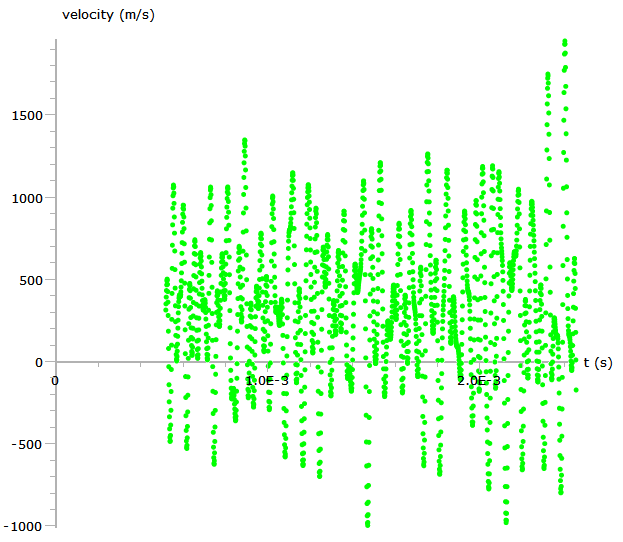
\includegraphics[width = 0.5\textwidth]{spin_10.png}
\caption{A graph of the calculated value of $\omega$ where loft is $10^{\circ}$}
\label{fig:spin10}
\end{figure}

\subsubsection{Spin}
To comment on Table \ref{spin} on spin of the ball. The spins (except for the spin of the $60^{\circ}$ club) seem to accurately re\mbox{f}lect the trend that as the loft of the club goes up, the ball spins more. The values of the spins themselves actually do agree quite well with measured values. When testing spins of balls \textit{Golf Magazine} used a Sand Wedge (about $55^{\circ}$ of loft), found values between 13,000 and 5,000 rpm for the golf balls tested. Therefore, the measured values $\sim$ 14,000--15,000 rpm at $60^{\circ}$ and $50^{\circ}$ respectively seem very reasonble. One note regarding the calculation of the spin: Because each individual ball oscillated somewhat randomly, the values of $\omega$ calculated can range wildly, as seen in Figure \ref{fig:spin10}. The true value of the spin can be found well be taking the average of points collected over the time interval.

\section{Conclusion}

The simulations conducted support the idea that a ball-spring model is an accurate approximation of a solid. While the ball-spring model can be more readily applied to prisms, where structure can be approximated as a lattice, as shown through this simulation, an approximation of a ball is equally valid. Results did not necessarily correspond perfectly to reality, but in general, trends seemed to be appropriate.

While the question of whether using dif\mbox{f}erent balls would af\mbox{f}ect spin was proposed, this question proved unreasonable to investigate. Firstly, the lack of data present on Young's moduli of various golf balls would have made an estimate required to continue. Similarly, after constructing the ball-spring model of the golf ball, it seemed unlike that the model could accurately capture such subtle tweaks in composition and structure. Thus, it was decided to investigate a simpler topic, where more data were available.

While the model created performed rather well given its complexity, many improvements could be made. To allow for more precision, a larger number of layerss could have been made. This would make the model more realistic in terms of composition. While a smaller time step could have been used, it seems unlikely that a smaller time step would benefit the simulation with significantly increased accuracy. It would be interesting to try and implement a dynamic coef\mbox{f}icient of restitution, one that decreases with more compression, to attempt to bring the ball speed into line with measurements. 

Many questions also remain to be investigated. For example, while an icosahedron was chosen as the base platonic solid in this model, would choosing a dif\mbox{f}erent solid, like a tetrahedron or octahedron, lead to dif\mbox{f}erent results? Another investigation lies in the idea of changing how cross-sectional area used to calculate the spring-constant is calculated. Currently, cross sectional area is simply the rest length squared. While this makes sense for a prism shape, it is harder to visualize how exactly it works in a sphere. Is there a better way to calculate cross sectional area for each spring? On the topic of springs, connecting each layer $L_{i}$ to every outer layer $L_{i + 1}$ involves using a set of connections that make sense but are not the only way to connect two layers. Would changing how the connections between layers are configured lead to a more accurate model? Finally, what would happen if the ball-spring model was abandoned all together, and instead of springs, forces based on the Lennard-Jones potential were used?

\appendix
\section{How to use the included code}
The code is designed to be as easy to modify and readable as possible. Therefore, a large list of constants (some of which should not be modified) is provided at the beginning of the file. It is recommended to try changing \texttt{LOFT} and \texttt{CLUB\_V0}. \texttt{SPIN} and \texttt{VELOCITY} determine which graphs are created, \texttt{DEBUG} will print some helpful messages and will by default allow stepping through the creation of the model and the animation.

Keyboard commands are also supported. \texttt{f} functions as a ``Play/Pause'' button for the animation, \texttt{s} will move through the animation and model creation one step at a time, and \texttt{b} will end the animation.

\section{The code}
\begin{verbatim}
##################################################################
##################################################################
## MODELING THE DEFORMATION OF A GOLF BALL
## a project for Physics 160 by Kar Epker
##################################################################
##################################################################

import collections
from visual import *
from visual.graph import *

##################################################################
## CONSTANTS
##################################################################

# simulation
DEBUG = False
LABEL = False
CURVES = True # turn off curve drawing between points
DT_BASIS = 1e-6

# keystrokes recognized
PLAY_STROKE = "f" # will play/pause animation
STEP_STROKE = "s" # will step through animation
BREAK_STROKE = "b" # will end animation

# golf ball properties
TOTAL_MASS = 45.93/1000 # in grams/1000 = kg
PARTICLE_MASS = TOTAL_MASS/217
YOUNG_MODULUS = 3.92e7
USE_BALL = False
RADIUS = 0.021
DEFAULT_NEIGHBOR_MODULUS = [2.94e8, 3.92e8, 3.92e8]
DEFAULT_LAYER_MODULUS = [3.92e7, 3.92e7, 3.92e7]
PIECES = 2 # cannot be more than length of layer/neighbor modulus

if USE_BALL: # data for a Callaway golf ball
    PIECE_RADII = [0.02100, 0.018798, 0.01194]
    NEIGHBOR_MODULUS = [2.94e8, 3.92e7, 3.92e7]
    LAYER_MODULUS = [3.92e7, 3.92e7, 3.92e7]

# particle properties
PARTICLE_RADIUS = RADIUS/100
CURVE_RADIUS = 3 * RADIUS/1000
PARTICLE_V0 = vector(0, 0, 0)

# model creation
SHAPE = "i" # icosahedron DO NOT CHANGE
FACES = 20 # DO NOT CHANGE
VERTS = 12 # DO NOT CHANGE
GEO_M = 1 # this m and n are valid for Class I geodesic spheres DO NOT CHANGE
GEO_N = 0
NEIGHBOR_TOLERANCE = 1.15 # should be 1 + (%tolerance/100)
LAYERS = PIECES + 1

# environment
A_G = 9.8
FNET_DAMP = 0.78 # from source

# club
CLUB_DEPTH = 5 * RADIUS/1000
CLUB_SIDE = RADIUS * 2.2
CLUB_R0 = vector(-RADIUS * 1.4, -RADIUS * 0.25, 0.0)
CLUB_V0 = vector(64.82, 0.0, 0.0)
CONTACT_TOLERANCE = 1.15 # should be 1 + (%tolerance/100)
CLUB_COLOR = (0.99, 0.99, 0.99)
LOFT = 0 # Degrees

# appearance
scene.background = color.white
scene.foreground = color.black
scene.width = 700
scene.height = 700
scene.center = vector(0, 0, 0)
scene.range = 3/2 * RADIUS * vector(1, 1, 1)

# graphs
SPIN = False # whether to make the spin graph
VELOCITIES = True # whether to make the velocity graph

display1 = gdisplay(x = 500, y = 0, width = 600, height = 600, background = color.white,
                    foreground = color.black, xtitle = "t (s)", ytitle = "velocity (m/s)",
                    title = "Velocity (m/s) vs. time")

v_com = gdots(gdisplay = display1, color = color.yellow)
spin = gdots(gdisplay = display1, color = color.green)
v_center = gdots(gdisplay = display1, color = color.blue)

##################################################################
## CLASSES
##################################################################

class Spring:
    neighbor = -1
    relation = ""
    rest = 0
    constant = 0
    modulus = 0
    def __init__(self, ind, rel, r, y, young = True):
        self.neighbor = ind
        self.relation = rel
        self.rest = r
        if young:
            self.modulus = y
            self.constant = (y * (r ** 2)) / r
        else:
            self.constant = y


##################################################################
## GEODESIC SPHERE CREATION, by Adrian Rossiter, adapted by Kar Epker
##################################################################
# vector functions

# convert numpy 2D array of form [n, 3] to 1D array of form [(x1, y1, z1), ... , (xn, yn, zn)]
def np_to_array(np):
    to_return = []
    for i in range(np.shape[0]):
        entry = (np[i, 0], np[i, 1], np[i, 2])
        to_return.append(entry)
    return to_return

# v0 + v1
def vec_add(v0, v1):
    return (v0[0]+v1[0], v0[1]+v1[1], v0[2]+v1[2])

# v0 - v1
def vec_subtract(v0, v1):
    return (v0[0]-v1[0], v0[1]-v1[1], v0[2]-v1[2])

# s * v0
def vec_scale(v0, s):
    return (s*v0[0], s*v0[1], s*v0[2])

# length v0
def vec_len(v0):
    return math.sqrt(v0[0]*v0[0] + v0[1]*v0[1] +v0[2]*v0[2])

# cross product v0xv1
def vec_cross(v0, v1):
    return (v1[2]*v0[1] - v1[1]*v0[2], v1[0]*v0[2] - v1[2]*v0[0], v1[1]*v0[0] - v1[0]*v0[1])

# scalar product v0.v1
def vec_scalar(v0, v1):
    return v0[0]*v1[0] + v0[1]*v1[1] + v0[2]*v1[2]


# individual shape functions

def get_octahedron(verts, faces):
    X = 0.25*math.sqrt(2)
    verts.extend( [ (0.0, 0.5, 0.0), (X, 0.0, -X), (X, 0.0, X), (-X, 0.0, X),
                   (-X, 0.0, -X), (0.0, -0.5, 0.0) ] )

    faces.extend( [ (0, 1, 2), (0, 2, 3), (0, 3, 4), (0, 4, 1),
                   (5, 2, 1), (2, 5, 3), (3, 5, 4), (4, 5, 1) ] )


def get_tetrahedron(verts, faces):
    X = 1/math.sqrt(3)
    verts.extend( [ (-X, X, -X), (-X, -X, X), (X, X, X), (X, -X, -X) ] )
    faces.extend( [ (0, 1, 2), (0, 3, 1), (0, 2, 3), (2, 1, 3) ] )
   

def get_triangle(verts, faces):
    if 1:
        Y = math.sqrt(3.0)/12.0
        Z = -0.8
        verts.extend( [(-0.25, -Y, Z), (0.25, -Y, Z), (0.0, 2*Y, Z) ] ) 
        faces.extend( [ (0, 1, 2) ] )
    else:
        X = .525731112119133606 
        Z = .850650808352039932
        verts.extend( [(-X, 0.0, -Z), (X, 0.0, -Z), (0.0, Z, -X), (0.0, -Z, -X)]) 
        faces.extend( [(0, 1, 2), (0, 3, 1)] )


def get_icosahedron(verts, faces):
   X = .525731112119133606 
   Z = .850650808352039932

   verts.extend([(-X, 0.0, Z), (X, 0.0, Z), (-X, 0.0, -Z), (X, 0.0, -Z),
                 (0.0, Z, X), (0.0, Z, -X), (0.0, -Z, X), (0.0, -Z, -X),
                 (Z, X, 0.0), (-Z, X, 0.0), (Z, -X, 0.0), (-Z, -X, 0.0)]) 

   faces.extend([(0, 4, 1), (0, 9, 4), (9, 5, 4), (4, 5, 8), (4, 8, 1),
                 (8, 10, 1), (8, 3, 10), (5, 3, 8), (5, 2, 3), (2, 7, 3),
                 (7, 10, 3), (7, 6, 10), (7, 11, 6), (11, 0, 6), (0, 1, 6),
                 (6, 1, 10), (9, 0, 11), (9, 11, 2), (9, 2, 5), (7, 2, 11)])


# determine which polygon to create

def get_poly(poly, verts, edges, faces):
    if poly=="i":
        get_icosahedron(verts, faces)
    elif poly=="o":
        get_octahedron(verts, faces)
    elif poly=="t":
        get_tetrahedron(verts, faces)
    elif poly=="T":
        get_triangle(verts, faces)
    else:
        return 0

    for face in faces:
        for i in range(0, len(face)):
            i2 = i+1
            if(i2==len(face)):
                i2=0
         
        if face[i] < face[i2]:
            edges[(face[i], face[i2])]=0
        else:
            edges[(face[i2], face[i])]=0

    return 1

# create and arrange points

def sphere_projection(points):
    for i in range(len(points)):
        points[i]= vec_scale(points[i], 1.0/vec_len(points[i]))


def grid_to_points(grid, freq, div_by_len, f_verts, face):
    f_verts = np_to_array(f_verts)
    points = []
    v = []
    for vtx in range(3):
        v.append([(0.0, 0.0, 0.0)])
        edge_vec = vec_subtract(f_verts[(vtx+1)%3], f_verts[vtx])
        if div_by_len:
            for i in range(1, freq+1):
                v[vtx].append(vec_scale(edge_vec, float(i)/freq))
        else:
            ang = 2*math.asin(vec_len(edge_vec)/2.0)
            unit_edge_vec = vec_scale(edge_vec, 1.0/vec_len(edge_vec))
            for i in range(1, freq+1):
                length = math.sin(i*ang/freq)/math.sin(math.pi/2 + ang/2 - i*ang/freq)
                v[vtx].append(vec_scale(unit_edge_vec, length))

    for (i, j) in grid.values():
        # skip vertex
        if (i==0) + (j==0) + (i+j==freq) == 2:
            continue

        # skip edges in one direction
        if (i==0 and face[2]>face[0]) or (j==0 and face[0]>face[1]) or (i+j==freq and face[1]>face[2]):
            continue

        n = [i, j, freq - i - j]
        v_delta = vec_add(v[0][n[0]], vec_subtract(v[(0-1)%3][freq-n[(0+1)%3]], v[(0-1)%3][freq]))
        pt = vec_add(f_verts[0], v_delta)
        if not div_by_len:
            for k in [1, 2]:
                v_delta = vec_add(v[k][n[k]], vec_subtract(v[(k-1)%3][freq-n[(k+1)%3]], v[(k-1)%3][freq]))
                pt = vec_add(pt, vec_add(f_verts[k], v_delta))
            pt = vec_scale(pt, 1.0/3)
        points.append(pt)

    return points


def make_grid(freq, m, n):
    grid = collections.OrderedDict() # changed this to use Ordered dict instead of dict
    for i in range(int(2*freq/(m+n))): # changed this to cast result to an int
        for j in range(int(2*freq/(m+n))):
            x = i*(-n) + j*(m+n)
            y = i*(m+n) + j*(-m)

            if x>=0 and y>=0 and x+y <= freq:
                grid[(i,j)] = (x, y)

    return grid

def make_sphere(shape, frequency, m, n):
    verts = []
    edges = {}
    faces = []
    get_poly(SHAPE, verts, edges, faces)
    verts = array(verts)

    grid = {}
    grid = make_grid(frequency * (m**2 + m * n + n**2), 1, 0)

    points = array(verts)

    for row in faces:
        if "i" == "T":
            face_edges = (0, 0, 0) # generate points for all edges
        else:
            face_edges = row

        new_points = grid_to_points(grid, frequency, 0, array([verts[row[i]] for i in range(3)]), face_edges)
        np_new_points = array(new_points)

        if not len(new_points) == 0: # don't append if there are no new points
            points = append(points, np_new_points, axis = 0)

    sphere_projection(points)

    return points

# end geodesic sphere creation
##################################################################

##################################################################
## INITIALIZATIONS
##################################################################

# connect the layers to each other
def connect_layers(particles, layers, modulus):

    # get threshold
    threshold = mag(particles[layers[-3]].pos - particles[layers[-2]].pos) * NEIGHBOR_TOLERANCE
    if layers[-1] - layers[-2] >= VERTS:
        threshold = mag(particles[layers[-3] + VERTS].pos - particles[layers[-2]].pos) * NEIGHBOR_TOLERANCE

    if DEBUG:
        print("connecting " + str(layers[-1] - layers[-2]) + " to outer layer within " + str(threshold))
        
    for outer in range(layers[-2], layers[-1]): # inner layer
        for inner in range(layers[-3], layers[-2]): # outer layer
            
            distance = mag(particles[outer].pos - particles[inner].pos)
            
            if outer == inner and DEBUG: # INVARIANT: outer should never equal inner
                raise AssertionError("two points in the same layer are trying to be connected")
            
            elif distance < threshold: # they are neighbors
                
                particles[outer].springs.append(Spring(inner, "nested", distance, modulus, True))
                particles[inner].springs.append(Spring(outer, "nested", distance, modulus, True))
        

# connect the adjacent vertices within each layer to each other 
def connect_neighbors(particles, start, modulus):

    # get threshold    
    threshold = mag(particles[start + 5].pos - particles[start + 4].pos) * NEIGHBOR_TOLERANCE
    if len(particles) - start > 14:
        threshold = mag(particles[start + VERTS + 1].pos - particles[start + VERTS].pos) * NEIGHBOR_TOLERANCE

    if DEBUG:
        print("connecting " + str(len(particles) - start) + " neighbors within " + str(threshold))
    
    for outer in range(start, len(particles)): # every particle in this layer
        for inner in range(start, len(particles)): # every other particle in this layer
            
            distance = mag(particles[outer].pos - particles[inner].pos)

            if outer == inner: # they are the same
                continue
            
            elif distance < threshold: # they are neighbors
                
                # although the relation is symmetric, only add one side for speed and coding ease
                particles[outer].springs.append(Spring(inner, "neighbor", distance, modulus, True))
         

def draw_sphere(points, particle_color, add_label = False):
    
    # initializations
    labels = []
    particles = []
    current_point = 0
    running = False
    last_stroke = ""

    while current_point < points.shape[0]: # while there are still points to place

        if scene.kb.keys: # keypress detection
            stroke = scene.kb.getkey()
            
            if stroke == PLAY_STROKE or stroke == STEP_STROKE: # if play/pause or step
                running = True
                last_stroke = stroke

        # make a VPython "sphere" object and append to list
        if running or not DEBUG:
            point = points[current_point]
            particles.append(sphere(radius = PARTICLE_RADIUS, pos = vector(point[0], point[1], point[2]),
                                    velocity = PARTICLE_V0, mass = PARTICLE_MASS, color = particle_color,
                                    springs = [], update = "", store = None))
            particles[-1].momentum = particles[-1].mass * particles[-1].velocity

            # label the points
            if DEBUG and LABEL:
                labels.append(label(pos = particles[current_point].pos, text = str(int(current_point))))

            # set values for next iteration
            current_point += 1
            if last_stroke == STEP_STROKE:
                running = False

    return particles

# get the radius for each layer
def get_properties():
    properties = {}
    piece_radii = []
    neighbor_modulus = []
    layer_modulus = []
    
    # if a ball is given
    if USE_BALL:
        properties['piece_radii'] = PIECE_RADII
        properties['neighbor_modulus'] = NEIGHBOR_MODULUS
        properties['layer_modulus'] = LAYER_MODULUS

    # default values
    else:   
        properties['piece_radii'] = linspace(1.0, 0.0, num = LAYERS) * RADIUS
        properties['neighbor_modulus'] = DEFAULT_NEIGHBOR_MODULUS
        properties['layer_modulus'] = DEFAULT_LAYER_MODULUS

    return properties


# make particle-spring model
def make_model():
    freq = 2**(LAYERS - 2)

    properties = get_properties()
    scales = properties['piece_radii']
    neighbor_modulus = properties['neighbor_modulus']
    layer_modulus = properties['layer_modulus']
    neighbor_counter = 0
    layer_counter = 0
    colors = [color.blue, color.yellow, color.orange, color.red]
    counter = 0
    
    points = empty(shape = (0, 3))
    particles = []
    layers = [0]
    
    # for each nested sphere
    while freq >= 1:
        if DEBUG:
            print("Layer " + str(counter) + " with freq " + str(int(freq)))
        
        # get and scale points
        new_points = make_sphere(SHAPE, int(freq), GEO_M, GEO_N)
        new_points *= scales[counter]
        points = append(points, new_points, axis = 0)

        # make and append set of VPython "sphere" objects for this layer
        new_particles = draw_sphere(new_points, colors[counter])
        particles.extend(new_particles)

        # keep track of indidces at which different layers start
        layers.append(layers[-1] + len(new_particles))
                          
        # connect layer to neighbors and outer layer if applicable
        connect_neighbors(particles, layers[counter], neighbor_modulus[neighbor_counter])
        neighbor_counter += 1
        if counter > 0:
            connect_layers(particles, layers, layer_modulus[layer_counter])
            layer_counter += 1
        
        # set values for the next loop
        if freq == 1:
            freq = 0
        else:
            freq /= 2
        counter += 1

    # last iteration for freq == -1 (single point) is a special case
    new_points = array([[0., 0., 0.]])
    new_particles = draw_sphere(new_points, colors[counter], LABEL)
    particles.extend(new_particles)
    layers.append(layers[-1] + len(new_particles))
    connect_layers(particles, layers, layer_modulus[layer_counter])

    return particles

# make the array of curves for the particle
def make_curves(particles):
    curves = []

    # at every spot in the array, make another array to hold curves
    for outer in range(len(particles)):
        particle = particles[outer]
        curves.append([])
        
        for spring in particle.springs:

            # determine color of curve
            curve_color = color.magenta
            if spring.relation == "neighbor":
                curve_color = particle.color
            
            curves[outer].append(curve(pos = [particle.pos, particles[spring.neighbor].pos],
                                radius = CURVE_RADIUS, color = curve_color))

    return curves

# reset
def reset():
    
    scene_info = {}

    # make the particle and club
    particles = make_model()
    club = box(length = CLUB_DEPTH, width = CLUB_SIDE, height = CLUB_SIDE,
               color = CLUB_COLOR, pos = CLUB_R0, velocity = CLUB_V0)
    get_club_plane(club)

    if CURVES: # make curves if drawing curves
        curves = make_curves(particles)
        scene_info['curves'] = curves

    scene_info['particles'] = particles
    scene_info['club'] = club
    
    return scene_info

# end initialization
##################################################################

##################################################################
## ANIMATION
##################################################################

# find normal vector and point on a club to determine the equation for its plane
def get_club_plane(club):

    # special case for if atan() is infinite
    if club.velocity.x == 0:
        club.norm = vector(cos(LOFT), sin(LOFT), 0)

    # for any other case of atan()
    else:
        phi = atan(club.velocity.y/club.velocity.x)
        club.norm = vector(1, 0, 0) # assume x component is 1
        club.norm.y = tan(radians(LOFT) - phi) * club.norm.x
        club.norm = norm(club.norm)

    # set visible attributes
    club.point = club.pos
    club.axis = club.norm
    club.length = CLUB_DEPTH

# general function for the momentum principle
def update_momentum(particle, Fnet, dt):

    particle.momentum += Fnet * dt
    particle.velocity = particle.momentum/particle.mass
    old_pos = particle.pos
    particle.pos += particle.velocity * dt

# update the position/properties of the particle based on the club's position
def update_club(particle, club):
    particle.pos = find_nearest_point(particle.pos, club)
    particle.velocity = club.velocity
    particle.momentum = particle.mass * particle.velocity

# find nearest point on the plane of the club to particle's position
# solve a(x + at) + b(y + bt) + c(z + ct) = d for t
# then nearest point is: = (x + at, y + bt, z + ct)
# where ax + by + cz = d is eq of plane, (x, y, z) is point
def find_nearest_point(point, club):
    
    # compute d and t
    d = dot(club.norm, club.pos)
    t = (d - (dot(club.norm, point)))/mag2(club.norm)

    # solve for point
    xp = point.x + club.norm.x * t
    yp = point.y + club.norm.y * t
    zp = point.z + club.norm.z * t

    return vector(xp, yp, zp)

# determine which way the particle's position will be updated
# using the club or using the momentum principle
def determine_update_method(particles, club, dt):

    # loop over all particles in the array
    for particle in particles:
        
        # calculate force from each spring and put in array
        forces = []
        for spring in particle.springs:
            stretch = mag(particle.pos - particles[spring.neighbor].pos) - spring.rest
            Fspring = -spring.constant * stretch * norm(particle.pos - particles[spring.neighbor].pos)
            forces.append(Fspring)

        # vector addition of all forces in Fnet array
        Fnet = vector(0, 0, 0)
        for force in forces:
            Fnet += force
        Fnet *= FNET_DAMP

        # calculate the positions of the particle and club one dt in the future
        calc_particle_pos = particle.pos + ((particle.momentum + (Fnet * dt))/particle.mass * dt)
        calc_club_point = club.pos + club.velocity * dt

        # test for particle contact with plane and update accordingly
        actual = (dot(calc_particle_pos - calc_club_point, club.norm))/mag(club.norm)
        contact_threshold = particle.radius * CONTACT_TOLERANCE

        # if the particle is behind the plane
        if actual < -contact_threshold:
            particle.update = "club"

        # otherwise
        else:
            particle.update = "momentum"
            particle.store = Fnet
        

# animate a given particle
def animate_particles(particles, club, dt):

    # for convenience
    for particle in particles:

        # INVARIANT: particle.update must be either "momentum" or "club"
        if DEBUG and not (particle.update == "momentum" or particle.update == "club"):
            raise AssertionError("particle update = " + particle.update)
        
        # update based on momentum
        if particle.update == "momentum":
            update_momentum(particle, particle.store, dt)

        # update based on the club position
        else: # particle.update == "club"
            update_club(particle, club)

        # clean the particle's update and store variables
        particle.update = ""
        particle.store = None


# animate the club
def animate_club(club, dt):
    club.pos += club.velocity * dt

# update the position of each of the curves
def draw_curves(particles, curves):

    # for every particle in the array, draw a curve between it and all its neighbors
    for outer in range(len(particles)):
        particle = particles[outer]
        
        for inner in range(len(particle.springs)):
            spring = particle.springs[inner]

            # update position of corresponding curve
            current = curves[outer][inner]
            current.pos = [particle.pos, particles[spring.neighbor].pos]

    return curves

# display the time in the upper left hand corner of the display
def animate_time(pos, time, t, dt):
    time.text = "t = " + str(t + dt)
    time.pos = pos + vector(-RADIUS, 1.7 * RADIUS, -1.5 * RADIUS)

# animate all objects
def animate(club, particles, curves, time, t, dt):

    animate_time(particles[-1].pos, time, t, dt)

    # animate particles and club
    determine_update_method(particles, club, dt)
    animate_club(club, dt)
    animate_particles(particles, club, dt)

    # draw the curves
    if CURVES:
        draw_curves(particles, curves)

# end animation
##################################################################

##################################################################
## SIMULATION
##################################################################

# get velocity of the center of mass for plotting
def get_com(particles):
    
    # set initial variables
    v = vector(0, 0, 0)
    r = vector(0, 0, 0)
    total_mass = 0

    # for every particle in the array
    for particle in particles:

        # perform appopriate calculations
        r += particle.mass * particle.pos
        v += particle.mass * particle.velocity
        total_mass += particle.mass

    # return the velocity of the center of mass
    return {'vcom': v/total_mass, 'rcom': r/total_mass}

# detect if first and second have a change in sign
def change_in_sign(first, second):
    if first > 0 and second > 0:
        return False
    elif first < 0 and second < 0:
        return False
    elif first == 0:
        if second == 0:
            return False
        else:
            return True
    else:
        return True

# plot
def plot(particles, centers, changes, omegas, last_vec, t, dt):

    # for convenience
    edge = particles[11]
    center = particles[-1]

    # perform calculations
    com = get_com(particles)
    rcom = com['rcom']
    vcom = com['vcom']
    current_vec = norm(rcom - edge.pos)
    
    # take care of spin plotting
    if SPIN and len(changes) > 5:
        dtheta = acos(dot(last_vec, current_vec))
        if dot(cross(last_vec, current_vec), vector(0, 0, 1)) < 0:
            dtheta = -dtheta
        omega = dtheta/dt
        omegas = append(omegas, omega)
        last_vec = current_vec
        spin.plot(pos = (t, omega))
    
    # take care of velocity plotting
    centers.append(center.velocity)
    if len(centers) > 2:
        old_slope = mag(centers[-2]) - mag(centers[-3])
        slope = mag(centers[-1]) - mag(centers[-2])
        if change_in_sign(old_slope, slope):
            changes = append(changes, t)
    
    if VELOCITIES:
        v_com.plot(pos = (t, mag(vcom)))
        v_center.plot(pos = (t, mag(center.velocity)))

    plot_info = {}
    plot_info['rcom'] = rcom
    plot_info['vcom'] = vcom
    plot_info['current_vec'] = current_vec
    plot_info['changes'] = changes
    plot_info['omegas'] = omegas
    return plot_info

# driver
def main_loop():

    # set time variables
    t = 0
    dt_basis = DT_BASIS
    dt = dt_basis

    # get variables from initialization
    scene_info = reset()
    particles = scene_info['particles']
    club = scene_info['club']
    curves = []
    time = label(pos = particles[-1].pos + vector(-RADIUS, 1.7 * RADIUS, -1.5 * RADIUS),text = "t = " + str(t),
                 color = color.black)
    if CURVES:
        curves = scene_info['curves']

    # data to keep track of for plotting
    centers = []
    changes = array([])
    omegas = array([])
    last_vec = vector(0, 0, 0)

    # set loop variables
    running = not DEBUG
    last_stroke = ""
    particles[11].color = color.black
    particles[11].radius = PARTICLE_RADIUS  * 2
    
    while True:

        if scene.kb.keys: # keypress detection
            stroke = scene.kb.getkey()
            
            if stroke == PLAY_STROKE: # play/pause
                running = not running
                last_stroke = stroke
                
            elif stroke == STEP_STROKE: # step
                running = True
                last_stroke = stroke
                
            elif stroke == BREAK_STROKE: # break
                break

        if running: # animate

            # update scene properties
            scene.center = particles[-1].pos
            animate(club, particles, curves, time, t, dt)

            # update quantities that have been modified in plot
            plot_info = plot(particles, centers, changes, omegas, last_vec, t, dt)
            last_vec = plot_info['current_vec']
            changes = plot_info['changes']
            omegas = plot_info['omegas']
            t += dt

            # handle keystrokes and messages
            if last_stroke == STEP_STROKE:
                print("step complete", end = "\n\n")
                running = False

            elif last_stroke == PLAY_STROKE:
                print("running")

            last_stroke = ""

    # post processing
    if VELOCITIES:
        collision = changes[1] - changes[0]
        remove_first = changes[1:]        
        diffs = ediff1d(remove_first)
        print("collision is " + str(collision) + " average of diffs is " + str(average(diffs)))
        print("velocity is " + str(plot_info['vcom']))

    if SPIN:
        print("omega is " + str(average(omegas)))

# end simulation
##################################################################

# run it like a boss
main_loop()
\end{verbatim}

\bibliographystyle{plain}
\bibliography{refs}
\end{document}
